%%%%%%%%%%%%%%%%%%%%%%%%%%%%%%%%%%%%%%%%%%%%%%%%%%%%%%%%%%%%
%%% ELIFE ARTICLE TEMPLATE
%%%%%%%%%%%%%%%%%%%%%%%%%%%%%%%%%%%%%%%%%%%%%%%%%%%%%%%%%%%%
%%% PREAMBLE 
\documentclass[9pt,lineno]{elife}

\usepackage{lipsum} % Required to insert dummy text
\usepackage[version=4]{mhchem}
\usepackage{siunitx}

\usepackage{makecell} % Allow splitting table cells into multiple lines.
\usepackage[colorinlistoftodos]{todonotes} % To add todos.
\DeclareSIUnit\Molar{M}

%%%%%%%%%%%%%%%%%%%%%%%%%%%%%%%%%%%%%%%%%%%%%%%%%%%%%%%%%%%%
%%% ARTICLE SETUP
%%%%%%%%%%%%%%%%%%%%%%%%%%%%%%%%%%%%%%%%%%%%%%%%%%%%%%%%%%%%
\title{Benchmarking SMIRNOFF99Frosst using host-guest calculations}

\author[1]{David R. Slochower}
\author[2]{Niel M. Henriksen}
% \author[3]{Michael R. Shirts}
\author[5]{John D. Chodera}
% \author[4]{David L. Mobley}
\author[1]{Michael K. Gilson}

\affil[1]{Skaggs School of Pharmacy and Pharmaceutical Sciences, University of California, San Diego, La Jolla, CA 92093, USA}
\affil[2]{Atomwise, Inc., San Francisco, CA 94105, USA}
% \affil[3]{Department of Chemical and Biological Engineering, University of Colorado Boulder, Boulder, CO 80309}
% \affil[4]{Department of Pharmaceutical Sciences and Department of Chemistry, University of California, Irvine, CA 92697, USA}
\affil[5]{Computational and Systems Biology Program, Sloan Kettering Institute, Memorial Sloan Kettering Cancer Center, New York, NY 10065}

\corr{mgilson@ucsd.edu}{MKG}

\newif\ifdraft
\drafttrue
\ifdraft
 \newcommand{\drsnote}[1]{ {\textcolor{red} { [DRS: #1] }}}
\else
 \newcommand{\drsnote}[1]{}
\fi


%%%%%%%%%%%%%%%%%%%%%%%%%%%%%%%%%%%%%%%%%%%%%%%%%%%%%%%%%%%%
%%% ARTICLE START
%%%%%%%%%%%%%%%%%%%%%%%%%%%%%%%%%%%%%%%%%%%%%%%%%%%%%%%%%%%%

\begin{document}

\maketitle
\drsnote{I have only included authors who reviewed the outline; I'm willing to revisit this issue in the future.}

\begin{abstract}

\end{abstract}

\section{Introduction}

\section{Methods}
\subsection{Host-guest systems}

In this manuscript, we report the binding thermodynamics for 43 host-guest complexes which were experimentally characterized in \cite{rekharsky_thermodynamic_1997} and previously studied in \cite{henriksen_evaluating_2017}. The host molecules are $\alpha$- or $\beta$-cyclodextrin with guests that can be characterized by their functional group as either ammonium, carboxylate, or cyclic alcohol.

\subsection{Force field parameters}
Host-guest systems were parameterized with 



GAFF v1.7 from Niel
GAFF v2.1 from AMBER18.


A single glucose molecule with methoxy caps on the O1 and O4 alcohols... AM1-BCC partial charges and GAFF v.17 Lennard-Jones and valence parameters.

GAFF v2.1 

\subsection{Simulations}
GAFF v1.7 simulations were performed with AMBER16; GAFF v2.1 and SMIRNOFF99Frosst simulations were performed with AMBER18 molecular dynamics software.
\subsection{Thermodynamic calculations}
We used the attach-pull-release (APR) method as implemented in the open source package pAPRika, version 0.0.3.

A complete description of the APR method is described in \cite{henriksen_computational_2015}.

\section{Results}
SMIRNOFF99Frosst does as well as GAFF, despite far fewer numerical force field parameters.

Text.
\begin{figure}[tb]
\centering
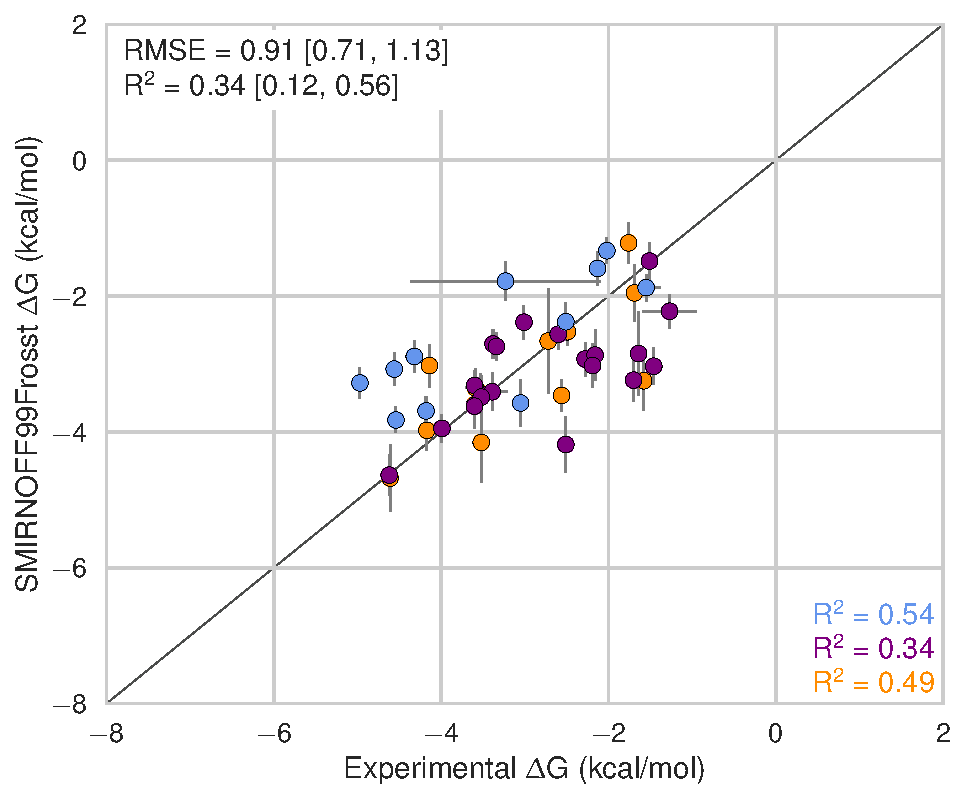
\includegraphics[width=0.5\textwidth]{images/SMIRNOFF99Frosst-vs-Experiment-dG.pdf}
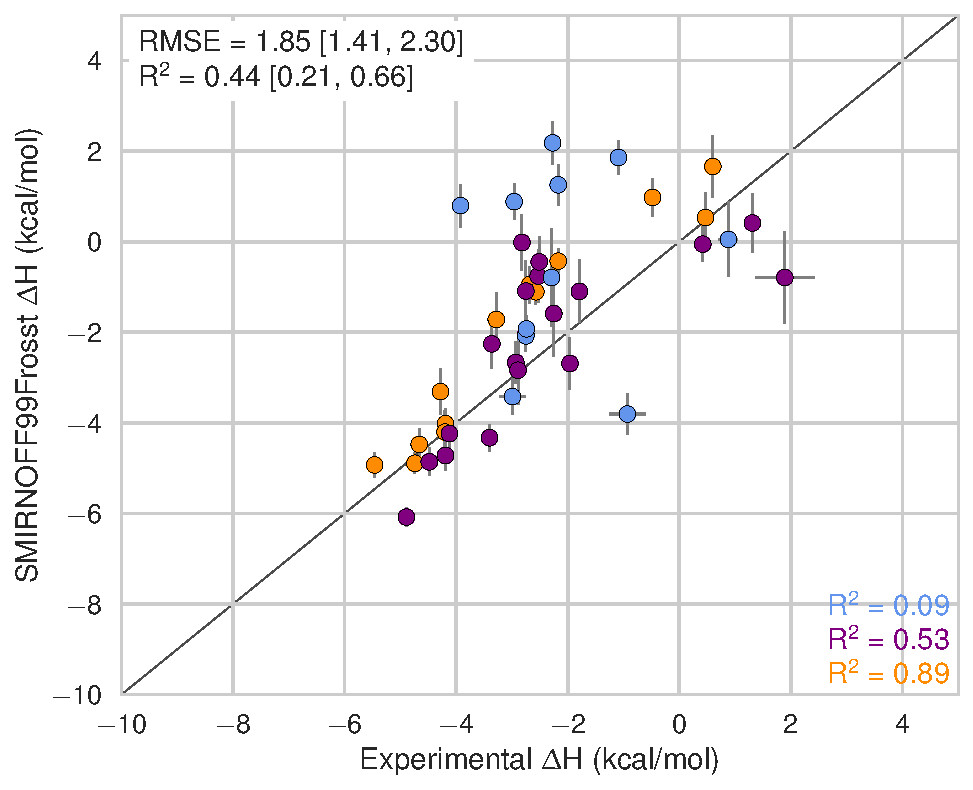
\includegraphics[width=0.5\textwidth]{images/SMIRNOFF99Frosst-vs-Experiment-dH.pdf}
\vspace{0.1cm}
\caption{Caption}
\label{fig:S99-vs-experiment}
\vspace{-0.6cm}
\end{figure}
Text.

\section{Discussion}

%%%%%%%%%%%%%%%%%%%%%%%%%%%%%%%%%%%%%%%%%%%%%%%%%%%%%%%%%%%%%%%%%%%%%%%%%%%%%%%%%%%%%%%%%%%%%%%%%%%%%%
% Code and Data Availability
%%%%%%%%%%%%%%%%%%%%%%%%%%%%%%%%%%%%%%%%%%%%%%%%%%%%%%%%%%%%%%%%%%%%%%%%%%%%%%%%%%%%%%%%%%%%%%%%%%%%%%

\section{Code and data availability}

%%%%%%%%%%%%%%%%%%%%%%%%%%%%%%%%%%%%%%%%%%%%%%%%%%%%%%%%%%%%%%%%%%%%%%%%%%%%%%%%%%%%%%%%%%%%%%%%%%%%%%
% Author Contributions 
%%%%%%%%%%%%%%%%%%%%%%%%%%%%%%%%%%%%%%%%%%%%%%%%%%%%%%%%%%%%%%%%%%%%%%%%%%%%%%%%%%%%%%%%%%%%%%%%%%%%%%
\section{Author Contributions}
Conceptualization, DRS, NMH, JDC, MKG; Methodology, DRS, NMH; Software, DRS, NMH; Formal Analysis, DRS, NMH, JDC, MKG; Investigation, DRS, NMH; Resources, MKG, JDC;  Data Curation, DRS, NMH; Writing-Original Draft, DRS, NMH; Writing - Review and Editing, DRS, NMH, JDC, MKG; Visualization, DRS; Supervision, JDC, MKG; Project Administration, MKG; Funding Acquisition, MKG.

%%%%%%%%%%%%%%%%%%%%%%%%%%%%%%%%%%%%%%%%%%%%%%%%%%%%%%%%%%%%%%%%%%%%%%%%%%%%%%%%%%%%%%%%%%%%%%%%%%%%%%
% Acknowledgments 
%%%%%%%%%%%%%%%%%%%%%%%%%%%%%%%%%%%%%%%%%%%%%%%%%%%%%%%%%%%%%%%%%%%%%%%%%%%%%%%%%%%%%%%%%%%%%%%%%%%%%%
\section{Acknowledgments}
The authors declare the following competing financial interest(s): MKG has an equity interest in and is a cofounder and scientific advisor of VeraChem LLC.
%%%%%%%%%%%%%%%%%%%%%%%%%%%%%%%%%%%%%%%%%%%%%%%%%%%%%%%%%%%%%%%%%%%%%%%%%%%%%%%%%%%%%%%%%%%%%%%%%%%%%%
% Disclosures 
%%%%%%%%%%%%%%%%%%%%%%%%%%%%%%%%%%%%%%%%%%%%%%%%%%%%%%%%%%%%%%%%%%%%%%%%%%%%%%%%%%%%%%%%%%%%%%%%%%%%%%
\section{Disclosures}

\bibliography{references}

%%%%%%%%%%%%%%%%%%%%%%%%%%%%%%%%%%%%%%%%%%%%%%%%%%%%%%%%%%%%
%%% APPENDICES
%%%%%%%%%%%%%%%%%%%%%%%%%%%%%%%%%%%%%%%%%%%%%%%%%%%%%%%%%%%%

\appendix
\section{List of abbreviations}
APR, attach-pull-release
\end{document}
